\chapter{Common Functions \& Operators: Math}



\section{Absolute Value ( $|x|$ )}\label{abs_value}
\begin{align*}
    \left| x \right| = \begin{cases}
       x & \text{ if\ } x \geq 0 \\
       -x & \text{ if\ } x < 0 
    \end{cases}
\end{align*}


\section{Factorial ( $x!$ )}\label{Factorial}
\[
    x! = \prod_{i=1}^{x} i = 1 \cdot 2 \cdots (x-1) \cdot x 
\]

\section{Combination ( $C(n,r)$ / $^nC_r$ / $nCr$ ) } \label{Combination}

\[
    C(n,r) = ^nC_r = nCr = \displaystyle\binom{n}{r} = \displaystyle\dfrac{n!}{(n-r)!r!}
\]

\section{Permutation \( \left(\ P(n,r)\ /\ ^nP_r\ /\ nPr\ \right) \)} \label{Permutation}

\[
    P(n,r) = ^nP_r = nPr = \displaystyle\dfrac{n!}{(n-r)!}
\]

\section{Exponential Function ( $exp(x)$ )}\label{Exponential Function}

\[
    exp(x) = e^x
\]

\section{Gamma Function ( $\Gamma(x)$ )}\label{Gamma Function}

\[
    \Gamma(x) = \dint_{0}^{\infty} t^{x-1} e^{-t} dt
\]


\section{Logarithm Function ( $\log(x)$ / $\ln(x)$ )}\label{Logarithm Function}
\[
    y = \log_a(x) \Leftrightarrow x = a^y
\]

Natural Logarithm Function ($a=e$):
\[
    y = \ln(x) \Leftrightarrow x = e^y
\]


\section{Sign Function ( $\rcmdXsgn(x)$ )}\label{Sign Function}
\begin{align*}
    \rcmdXsgn(x) = \begin{cases}
         1 & \text{ if } x > 0 \\
         0 & \text{ if } x = 0 \\
         -1 & \text{ if } x < 0 
        \end{cases}
\end{align*}



\section{Indicator function ( $\mathbbm{1}_x$ )}\label{Indicator function}

\begin{align*}
    \mathbbm{1}_x = {\begin{cases}
        1 & \text{ if x is true } \\
        0 & \text{ if x is false }
    \end{cases}}
\end{align*}

\section{Infinite Step Function ( $1(z)$ )}

\begin{align*}
    1(z) = {\begin{cases}
        0 & \text{ if } z \leq 0 \\
        \infty & \text{ otherwise }
    \end{cases}}
\end{align*}

This gives infinite penalty if the constraint is not satisfied.


\section{Trigonometric functions - TODO \cite{wiki-Trigonometric_functions}}\label{Trigonometric functions}

\begin{table}[H]
    \centering
    \begin{minipage}[t]{0.3\linewidth}
        \begin{figure}[H]
            \centering
            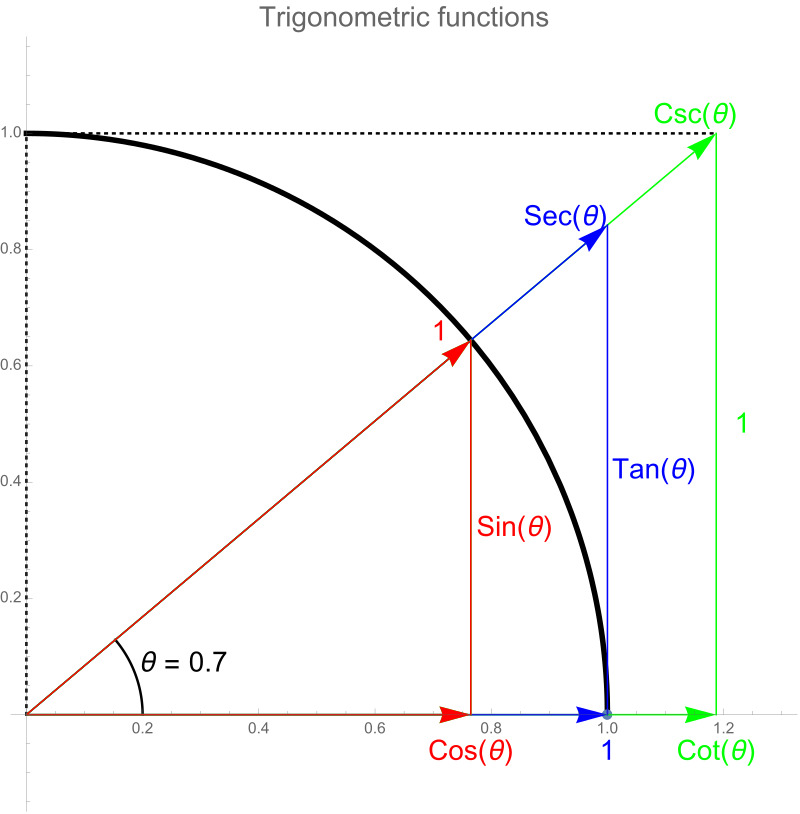
\includegraphics[height=4.5cm]{Pictures/maths/TrigFunctions.jpg}
            \caption{Trigonometry Functions Comparison}
        \end{figure}
    \end{minipage}
    \hfill
    \begin{minipage}[t]{0.3\linewidth}
        \begin{figure}[H]
            \centering
            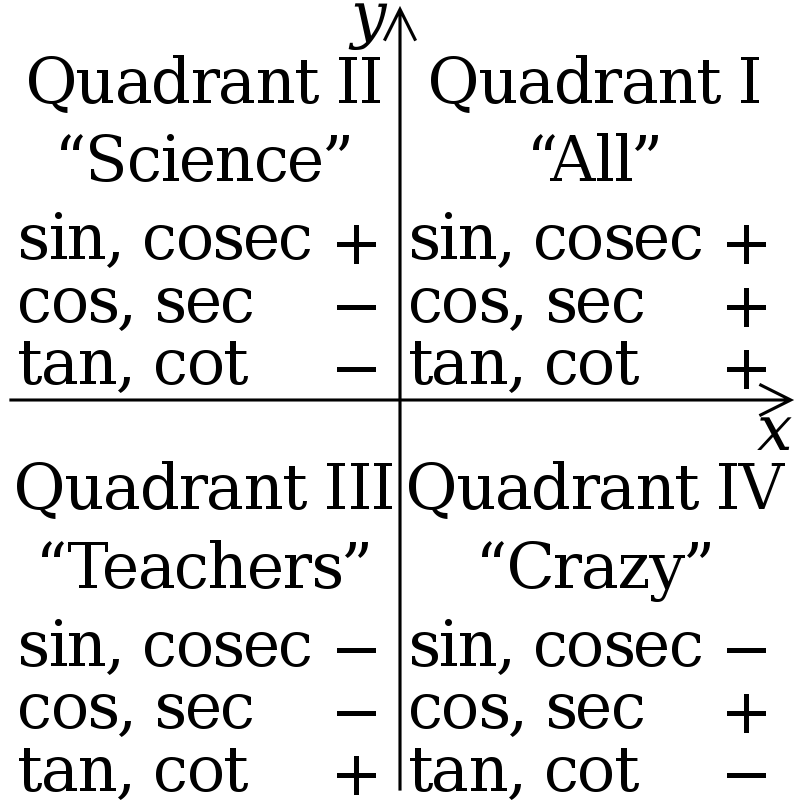
\includegraphics[height=4.5cm]{Pictures/maths/Trigonometric_function_quadrant_sign.png}
            \caption{Trigonometry Quadrant Signs}
        \end{figure}
    \end{minipage}
    \begin{minipage}[t]{0.3\linewidth}
        \begin{figure}[H]
            \centering
            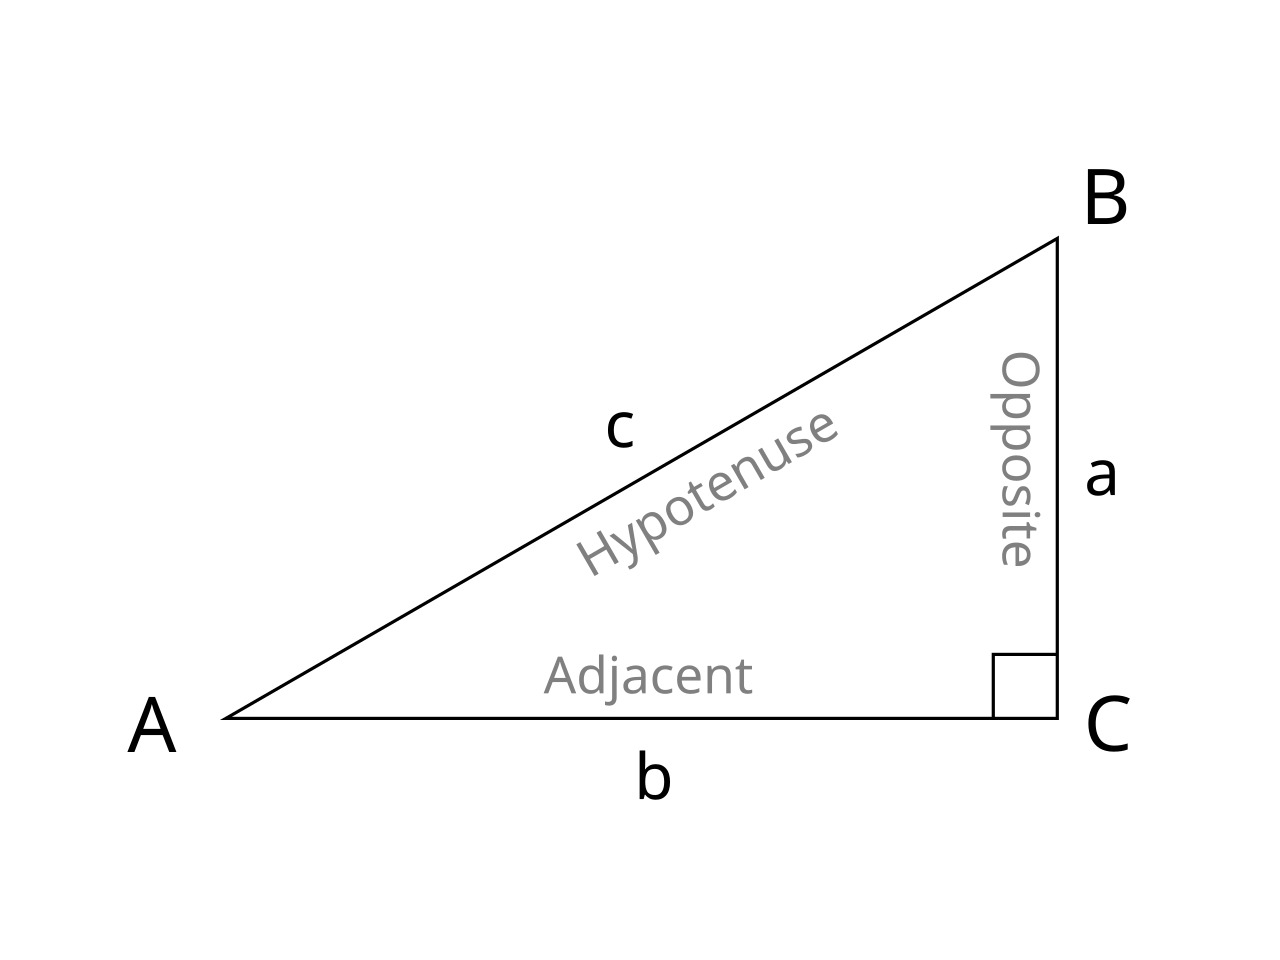
\includegraphics[height=4.5cm]{Pictures/maths/TrigonometryTriangle.jpg}
            \caption{Trigonometry Triangle}
        \end{figure}        
    \end{minipage}
\end{table}

\subsection{sine ( $\sin(\theta)$ )}\label{sine (sin)}

\[
    \sin(\theta) = \displaystyle \dfrac{\mathrm{opposite}}{\mathrm{hypotenuse}}
\]
\[    \sin(\theta + 2k\pi) = \sin(\theta)   \]

\subsection{cosine ( $\cos(\theta)$ )}\label{cosine (cos)}

\[
    \cos(\theta) = \displaystyle\dfrac{\mathrm {adjacent} }{\mathrm {hypotenuse} }
\]
\[  \cos(\theta + 2k\pi ) = \cos(\theta)  \]

\subsection{tangent ( $\tan(\theta)$ )}\label{tangent (tan)}

\[
    \tan(\theta) =\displaystyle \frac {\mathrm {opposite} }{\mathrm {adjacent} }
\]
\[  \tan(\theta + k\pi ) = \tan(\theta)  \]

\subsection{cosecant ( $\csc(\theta)$ }\label{cosecant (csc)}
\[
    \csc(\theta) =\displaystyle\frac {\mathrm {hypotenuse} }{\mathrm {opposite} }
\]

\subsection{secant ( $\sec(\theta)$ )}\label{secant (sec)}
\[
    \sec(\theta) =\displaystyle\frac {\mathrm {hypotenuse} }{\mathrm {adjacent} }
\]

\subsection{cotangent ( $\cot(\theta)$ )}\label{cotangent (cot)}

\[
    \cot(\theta) =\displaystyle\frac {\mathrm {adjacent} }{\mathrm {opposite} }
\]
\[  \cot(\theta + k\pi ) = \cot(\theta)  \]


\subsection{Properties \& Formulas}
\begin{enumerate}
    \item \( \sin^2(\theta) + \cos^2(\theta) = 1 \)
\end{enumerate}


\section{Inverse trigonometric functions - TODO \cite{wiki-Inverse_trigonometric_functions}}\label{Inverse trigonometric functions}

\section{Hyperbolic Functions \cite{wiki-Hyperbolic_functions}}\label{Hyperbolic functions}


\begin{table}[H]
    \centering
    \begin{minipage}[t]{0.45\linewidth}
        \begin{figure}[H]
            \centering
            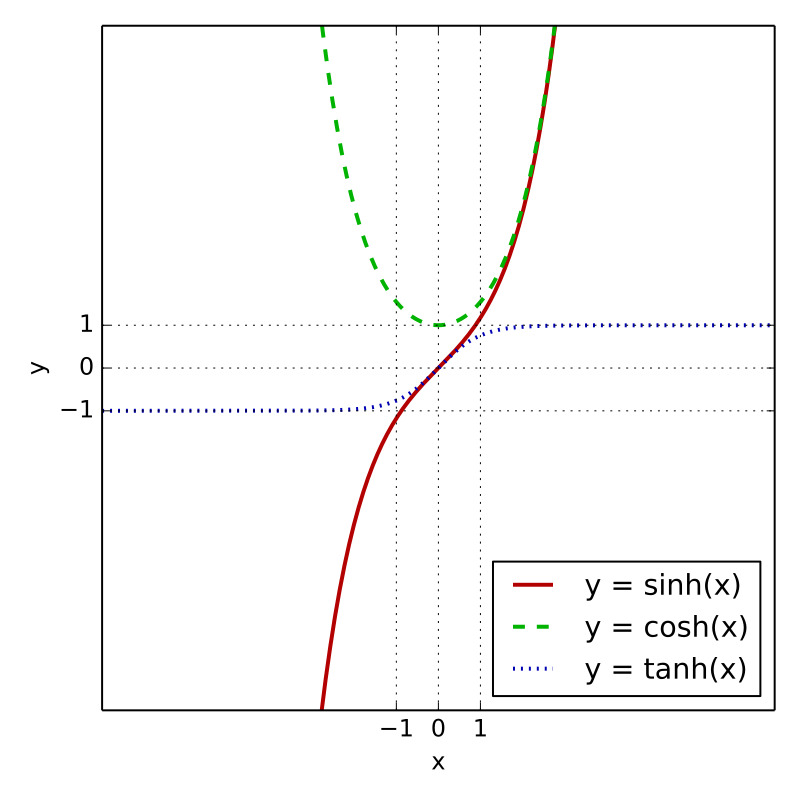
\includegraphics[height=7.5cm]{Pictures/maths/Sinh_cosh_tanh.jpg}
            \caption{$\sinh(x)$, $\cosh(x)$ \& $\tanh(x)$}
        \end{figure}        
    \end{minipage}
    \hfill
    \begin{minipage}[t]{0.45\linewidth}
        \begin{figure}[H]
            \centering
            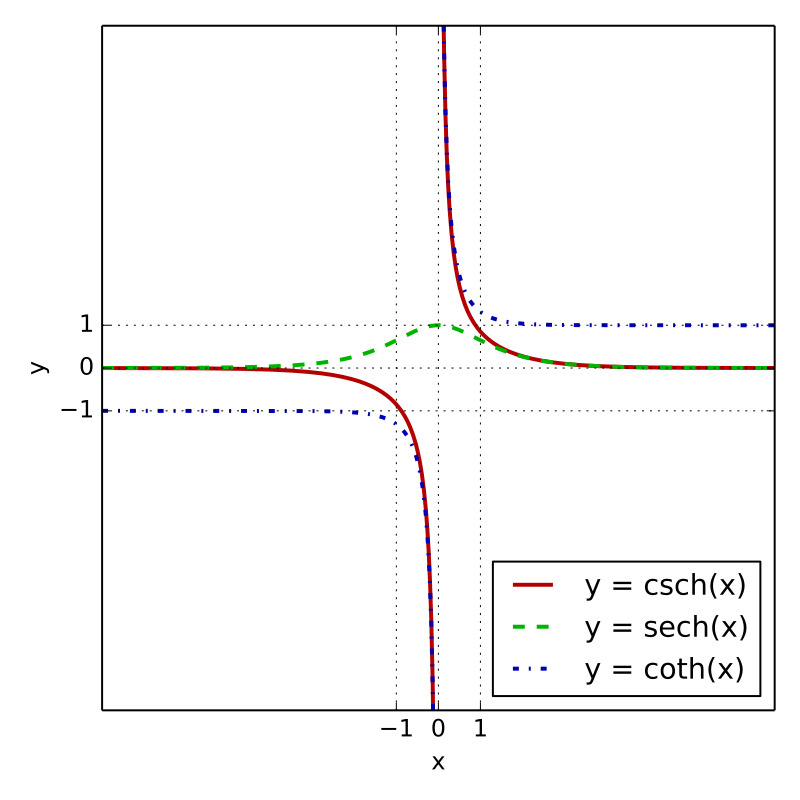
\includegraphics[height=7.5cm]{Pictures/maths/Csch_sech_coth.jpg}
            \caption{$\rcmdXcsch(x)$, $\rcmdXsech(x)$ \& $\coth(x)$}
        \end{figure}
    \end{minipage}
\end{table}

\subsection{Hyperbolic sine ( $\sinh(x)$ ) }\label{Hyperbolic sine (sinh)}
\[
    (\sinh(x) = {\displaystyle\dfrac{e^{x} - e^{-x}}{2}}={\displaystyle\dfrac{e^{2x} - 1}{2e^{x}}}={\displaystyle\dfrac{1 - e^{-2x}}{2e^{-x}}}
\]

\subsection{Hyperbolic cosine ( $\cosh(x)$ ) }\label{Hyperbolic cosine (cosh)}
\[
    \cosh(x) = {\displaystyle\dfrac{e^{x} + e^{-x}}{2}} = {\displaystyle\dfrac{e^{2x} + 1}{2e^{x}}} = {\displaystyle\dfrac{1 + e^{-2x}}{2e^{-x}}}
\]

\subsection{Hyperbolic tangent ( $\tanh(x)$ )}\label{Hyperbolic tangent (tanh)}
\[
    \tanh(x) = \displaystyle\dfrac{\sinh(x)}{\cosh(x)} = \displaystyle\dfrac{e^{x} - e^{-x}}{e^{x} + e^{-x}} = \displaystyle\dfrac{e^{2x} - 1}{e^{2x} + 1}
\]

\subsection{Hyperbolic cotangent ( $\coth(x)$ )}\label{Hyperbolic cotangent (coth)}
\[
    \coth(x) = \displaystyle\dfrac{1}{\tanh(x)} = \displaystyle\dfrac{\cosh(x)}{\sinh(x)} = \displaystyle\dfrac{e^{x} + e^{-x}}{e^{x} - e^{-x}} = \displaystyle\dfrac{e^{2x} + 1}{e^{2x} - 1}
\]

$x \neq 0$

\subsection{Hyperbolic secant ( $\rcmdXsech(x)$ )} \label{Hyperbolic secant (sech)}
\[
    \rcmdXsech(x) = \displaystyle\dfrac{1}{\cosh(x)} = \displaystyle\dfrac{2}{e^{x} + e^{-x}} = \displaystyle\dfrac{2e^{x}}{e^{2x} + 1}
\]

\subsection{Hyperbolic cosecant ( $\rcmdXcsch(x)$ )}\label{Hyperbolic cosecant (csch)}
\[
    \rcmdXcsch(x) = \displaystyle\dfrac{1}{\sinh(x)} = \displaystyle\dfrac{2}{e^{x} - e^{-x}} = \displaystyle\dfrac{2e^{x}}{e^{2x} - 1}
\]
$x \neq 0$

\subsection{Properties \& Formulas}

\begin{table}[H]
    \centering
    \begin{tabular}{|c|r|r|r|r|r|r|}
        \hline
        $\theta$ & $\sinh(\theta)$ & $\cosh(\theta)$ & $\tanh(\theta)$ & $\coth(\theta)$ & $\rcmdXsech(\theta)$ & $\rcmdXcsch(\theta)$ \\ \hline

        $-\theta$ & $-\sinh(\theta)$ & $\cosh(\theta)$ & $-\tanh(\theta)$ & $-\coth(\theta)$ & $\rcmdXsech(\theta)$ & $-\rcmdXcsch(\theta)$ \\ \hline
    \end{tabular}
    \caption{Hyperbolic angles}
\end{table}

\section{Softmax function ( $\sigma (\mathbf {z})$ ) \cite{wiki-softmax-function}}\label{Softmax function}
The softmax function, also known as softargmax or normalized exponential function, converts a vector of $K$ real numbers into a probability distribution of $K$ possible outcomes. It is a generalization of the logistic function to multiple dimensions, and used in multinomial logistic regression. The softmax function is often used as the last activation function of a neural network to normalize the output of a network to a probability distribution over predicted output classes.

\[
    {\displaystyle \sigma (\mathbf {z} )_{i}={\displaystyle\frac {e^{z_{i}}}{\sum _{j=1}^{K}e^{z_{j}}}}}
\]

Where:
\[
    {\displaystyle \sigma \colon \mathbb {R} ^{K}\to (0,1)^{K}}
    \hfill
    {\displaystyle K\geq 1}
\]
\[
    {\displaystyle \mathbf {z} =(z_{1},\dotsc ,z_{K})\in \mathbb {R} ^{K}}
\]





















































